\documentclass[10pt,twocolumn]{memoir}

% Left and right margins
\setlrmarginsandblock{0.35in}{0.35in}{*}

% Top and bottom margins
\setulmarginsandblock{1in}{0.8in}{*}

% Apply the layout
\checkandfixthelayout

% Space between the two columns
\setlength{\columnsep}{0.2in}

\usepackage{microtype}
\usepackage{mathpazo}
\usepackage{amsmath}
\usepackage{tikz}
\usetikzlibrary{arrows.meta}

\begin{document}

\appendix

\chapter{Calculus of Variations}
\label{app:calculus_of_variations}

We can think of a function $y(x)$ as being an operator that, for any input value $x$, returns an output value $y$. In the same way, we can define a functional $F[y]$ to be an operator that takes a function $y(x)$ and returns an scalar value $F$. An example of a functional is the length of a curve drawn in a two-dimensional plane in which the path of the curve is defined in terms of a function. In the context of machine learning, a widely used functional is the entropy $\mathrm{H}[x]$ for a continuous variable $x$ because, for any choice of probability density function $p(x)$, it returns a scalar value representing the entropy of $x$ under that density. Thus the entropy of $p(x)$ could equally well have been written as $\mathrm{H}[p]$.

A common problem in conventional calculus is to find a value of $x$ that maximizes (or minimizes) a function $y(x)$. Similarly, in the calculus of variations we seek a function $y(x)$ that maximizes (or minimizes) a functional $F[y]$. That is, of all possible functions $y(x)$, we wish to find the particular function for which the functional $F[y]$ is a maximum (or minimum). The calculus of variations can be used, for instance, to show that the shortest path between two points is a straight line or that the maximum entropy distribution is a Gaussian.

Using a Taylor expansion, we can characterize the conventional derivative $dy/dx$ by making a small change $\epsilon$ to the variable $x$ and expanding $y(x+\epsilon)$ about $x$:

\begin{equation}
    y(x+\epsilon) = y(x) + \frac{dy}{dx}\epsilon + O(\epsilon^2).
\label{eq:a4_single_variable_derivative}
\end{equation}

and finally taking the limit $\epsilon \to 0$. Similarly, for a function of several variables $y(x_1,\ldots,x_D)$, the corresponding partial derivatives are defined such that

\begin{equation}
    y(x_1+\epsilon_1,\ldots,x_D+\epsilon_D) = y(x_1,\ldots,x_D) + \sum_{i=1}^{D}\frac{\partial y}{\partial x_i}\epsilon_i + O(\epsilon^2).
\label{eq:a4_multivariate_derivative}
\end{equation}

The analogous definition of a functional derivative arises when we consider how much a functional $F[y]$ changes when we make a small change $\epsilon\eta(x)$ to the function $y(x)$, where $\eta(x)$ is an arbitrary function of $x$, as illustrated in Fig.~\ref{fig:functional_derivative}. We denote the functional derivative of $F[y]$ with respect to $y(x)$ by $\delta F/\delta y(x)$, and define it by the following relation:

\begin{equation}
    F[y(x) + \epsilon \eta(x)] = F[y(x)] + \epsilon\int\frac{\delta F}{\delta y(x)}\eta(x)\,dx + O(\epsilon^2).
\label{eq:a4_functional_derivative}
\end{equation}

\begin{figure}[t]
    \centering
    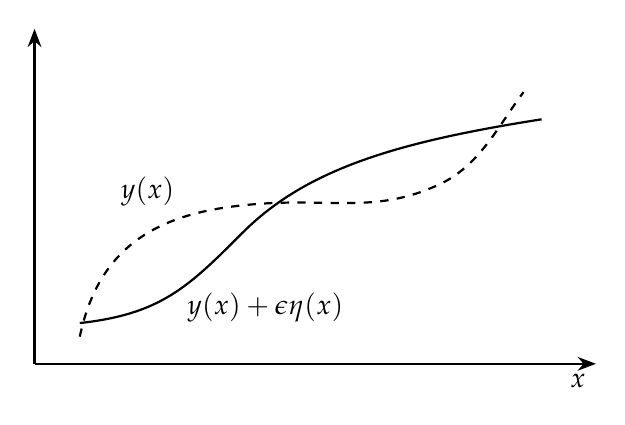
\begin{tikzpicture}[scale=1.15, >=Stealth]

        % Axes
        \draw[->, thick] (0,0) -- (6.2,0)
            node[below left] {$x$};
        \draw[->, thick] (0,0) -- (0,3.7);

        % y(x): solid black
        \draw[black, thick]
            (0.5,0.45)
            .. controls (1.4,0.55) and (1.7,0.85) .. (2.3,1.45)
            .. controls (3.0,2.15) and (4.0,2.45) .. (5.6,2.70);

        % y(x) + epsilon eta(x): dashed black
        \draw[black, thick, dashed]
            (0.5,0.30)
            .. controls (0.7,1.25) and (1.3,1.65) .. (2.3,1.75)
            .. controls (3.2,1.85) and (3.7,1.65) .. (4.4,1.95)
            .. controls (4.9,2.15) and (5.1,2.60) .. (5.4,3.00);

        % Labels
        \node[fill=white, inner sep=1pt] at (1.25,1.90) {$y(x)$};
        \node[fill=white, inner sep=1pt] at (2.55,0.62) {$y(x)+\epsilon\eta(x)$};

    \end{tikzpicture}

    \caption{A functional derivative can be defined by considering how the
    value of a functional $F[y]$ changes when the function $y(x)$ is changed
    to $y(x)+\epsilon\eta(x)$, where $\eta(x)$ is an arbitrary function of $x$.}
\label{fig:functional_derivative}
\end{figure}

This can be seen as a natural extension of \ref{eq:a4_multivariate_derivative} in which $F[y]$ now depends on a continuous set of variables, namely the values of $y$ at all points $x$.

If our goal is to find a function $y(x)$ that maximizes or minimizes the functional $F[y]$, we require $F[y]$ to be stationary at the optimal function. Here, stationarity means that an arbitrary small perturbation $y(x)\rightarrow y(x)+\epsilon\eta(x)$ produces no first-order change in $F[y]$. From Eq.~\ref{eq:a4_functional_derivative}, the coefficient of $\epsilon$ must therefore vanish, giving

\begin{equation}
    \int\frac{\delta F}{\delta y(x)}\eta(x)\,dx = 0.
\label{eq:a4_stationarity}
\end{equation}

Because this condition must hold for every possible perturbation $\eta(x)$, the functional derivative itself must be zero for all $x$. To see why, suppose that $\delta F/\delta y(x)$ were nonzero near some point $\hat{x}$. We could then choose $\eta(x)$ to be zero everywhere except in a small neighbourhood of $\hat{x}$, and choose its sign so that

\begin{equation}
    \frac{\delta F}{\delta y(x)}\eta(x) > 0
\end{equation}

throughout that neighbourhood. The integral in Eq.~\ref{eq:a4_stationarity} would then be positive rather than zero, which contradicts the stationarity condition. Therefore, $\delta F/\delta y(x)$ cannot be nonzero near any point, and we must have $\delta F/\delta y(x)=0$ for all values of $x$.

Consider a functional that is defined by an integral over a function $G(y,y',x)$ that depends on both $y(x)$ and its derivative $y'(x)$, as well as directly on $x$,

\begin{equation}
    F[y] = \int G\left(y(x),y'(x),x\right)\,dx.
\end{equation}

If we perturb the function according to $y(x)\rightarrow y(x)+\epsilon\eta(x)$, then its derivative is also perturbed according to $y'(x)\rightarrow y'(x)+\epsilon\eta'(x)$. Thus, the first two arguments of $G$ are perturbed, while the independent variable $x$ itself remains unchanged. For small $\epsilon$, we can therefore apply a multivariable Taylor expansion to the integrand,

\begin{equation}
    G(y+\epsilon\eta,y'+\epsilon\eta',x) = G(y,y',x) + \epsilon\frac{\partial G}{\partial y}\eta(x) + \epsilon\frac{\partial G}{\partial y'}\eta'(x) + O(\epsilon^2).
\end{equation}

Substituting this expansion of $G$ into the perturbed functional gives

\begin{equation}
\begin{aligned}
    F[y+\epsilon\eta]
    &= \int G\left(y+\epsilon\eta, y'+\epsilon\eta', x\right)\,dx. \\
    &= \int \left[G(y,y',x) + \epsilon\frac{\partial G}{\partial y}\eta(x) + \epsilon\frac{\partial G}{\partial y'}\eta'(x) + O(\epsilon^2)\right]dx \\
    &= F[y] + \epsilon\int\left[\frac{\partial G}{\partial y}\eta(x) + \frac{\partial G}{\partial y'}\eta'(x)\right]dx + O(\epsilon^2).
\end{aligned}
\end{equation}

There is no term involving $\partial G/\partial x$ because the perturbation changes the function $y(x)$, not the independent variable $x$.

We now have to cast this in the form Eq.~\ref{eq:a4_functional_derivative}. To do so, we need to express the first-order change in $F[y]$ entirely in terms of $\eta(x)$. However, the second term in the integral contains $\eta'(x)$. We therefore apply integration by parts,

\begin{equation}
    \int\frac{\partial G}{\partial y'}\eta'(x)\,dx = \left[\frac{\partial G}{\partial y'}\eta(x)\right]_{\mathrm{boundary}} - \int\frac{d}{dx}\left(\frac{\partial G}{\partial y'}\right)\eta(x)\,dx.
\end{equation}

Assume that we are only searching over all admissible functions $y(x)$ that connect fixed endpoint values. The perturbed function $y(x)+\epsilon\eta(x)$ must therefore have the same endpoint values as the original function $y(x)$. This requires $\eta(x)=0$ at the boundaries, so the boundary term vanishes, leaving

\begin{equation}
    \int \frac{\partial G}{\partial y'}\eta'(x)\,dx = -\int\frac{d}{dx}\left(\frac{\partial G}{\partial y'}\right)\eta(x)\,dx.
\end{equation}

Substituting this result into the first-order expansion of $F[y+\epsilon\eta]$ gives

\begin{equation}
    F[y+\epsilon\eta] = F[y] + \epsilon\int\left[\frac{\partial G}{\partial y} - \frac{d}{dx}\left(\frac{\partial G}{\partial y'}\right)\right]\eta(x)\,dx + O(\epsilon^2).
\end{equation}

This expression now has the same form as Eq.~\ref{eq:a4_functional_derivative}, so the quantity in square brackets can be identified as the functional derivative $\delta F/\delta y(x)$.

To find a function $y(x)$ at which the functional $F[y]$ is stationary, we require its functional derivative to be 0,

\begin{equation}
    \frac{\partial G}{\partial y} - \frac{d}{dx}\left(\frac{\partial G}{\partial y'}\right) = 0,
\label{eq:a4_euler_lagrange_equation}
\end{equation}

which are known as the \textit{Euler--Lagrange equation}. For example, if

\begin{equation}
    G = y(x)^2 + \left(y'(x)\right)^2
\end{equation}

then the Euler--Lagrange equations take the form

\begin{equation}
    y(x) - \frac{d^2y}{dx^2} = 0.
\end{equation}

The general solution to this second-order differential equation is

\begin{equation}
    y(x) = C_1 e^x + C_2 e^{-x},
\end{equation}

where the constants $C_1$ and $C_2$ are determined by the boundary values of $y(x)$.

Often, we consider functionals whose integrands take the form $G(y,x)$ and therefore do not depend on derivatives of $y(x)$. In this case, the Euler--Lagrange equation simplifies directly, and stationarity requires $\partial G / \partial y = 0$ for all values of $x$.

The extension to a multidimensional variable $\mathbf{x}$ is straightforward by applying the same reasoning componentwise. A small perturbation is now applied to a function $y(\mathbf{x})$, and ordinary derivatives with respect to $x$ are replaced by the corresponding partial derivatives with respect to the components of $\mathbf{x}$. Stationarity is then obtained by requiring the first-order change in the functional to vanish for arbitrary perturbations.

\end{document}
